\documentclass[11pt]{article}
\usepackage[top=2cm,left=2cm,right=2cm,bottom=2cm]{geometry}
\usepackage[doublespacing]{setspace}
\usepackage{graphicx}
\usepackage{xcolor}
\usepackage{subfigure}
\usepackage[hidelinks]{hyperref}
\usepackage{amsmath}
\usepackage{amssymb}
\usepackage{lscape}
\usepackage{booktabs}
\usepackage{listings}
\usepackage{pythonhighlight}
\usepackage{tcolorbox}
\usepackage[localise]{xepersian}
\settextfont{XB Niloofar}

\definecolor{codegreen}{rgb}{0,0.6,0}
\definecolor{codegray}{rgb}{0.5,0.5,0.5}
\definecolor{codepurple}{rgb}{0.58,0,0.82}
\definecolor{backcolour}{rgb}{0.95,0.95,0.92}

\lstdefinestyle{mystyle}{
	backgroundcolor=\color{backcolour},   
	commentstyle=\color{codegreen},
	keywordstyle=\color{magenta},
	numberstyle=\tiny\color{codegray},
	stringstyle=\color{codepurple},
	basicstyle=\ttfamily\footnotesize,
	breakatwhitespace=false,         
	breaklines=true,                 
	captionpos=b,                    
	keepspaces=true,                 
	numbers=left,                    
	numbersep=5pt,                  
	showspaces=false,                
	showstringspaces=false,
	showtabs=false,                  
	tabsize=2
}
\lstset{style=mystyle}

\begin{document}
	\شروع{وسط‌چین}
	به نام خدا\\
	\vspace{1cm}
	\begin{figure}[h]
		\begin{center}
			\includegraphics[width=0.3\linewidth]{"D:/Logo/UT"}
		\end{center}
	\end{figure}
	{\درشت‌درشت دانشکده مهندسی مکانیک}\\
	\vspace{1cm}
	{\بزرگ \سیاه{نام درس: هوش مصنوعی}}\\
	
	\vspace{0.5cm}
	{\درشت‌درشت تمرین ۵(یادگیری تقویتی)}
	\vspace{1.5cm}
	
	\vspace{1.5cm}
	{\درشت‌درشت {\سیاه استاد درس:} دکتر شریعت‌پناهی}\\
	\vspace{2cm}
	{\درشت‌درشت {\سیاه دانشجو:}}\\
	{\درشت مهدی نوذری\\
	810601139}\\
	\vspace{3cm}
	تابستان ۱۴۰۳\\
	\پایان{وسط‌چین}
	\pagebreak
		تمامی فایل‌ها در \lr{Github} موجود هستند:
	\href{https://github.com/Morphit/UT_AI_1403}{\lr{https://github.com/Morphit/UT\_AI\_1403}}
	
	\vspace{1cm}
	در این گزارش پیاده‌سازی الگوریتم‌های یادگیری تقویتی بر روی یک بازوی رباتیک انجام می‌شود. در طی این روند یک محیط تعریف شده که ساختار ربات و همجنین محیط اطراف آن را توصیف می‌کند. سپس با تعریف یک عامل به وسیله الگوریتم‌های مختلف، عامل‌ها سعی در پیدا کردن مسیر مناسب برای رسیدن به هدف از یک نقطه اولیه خواهند داشت.
	\section{تعریف محیط}
	محیطی که باید تعریف شود شامل ربات، هدف نهایی و موانع، و همچنین نحوه پاداش‌دهی به عامل می‌باشد. در این تمرین از یک ربات با ساختار مشابه ربات 
	\lr{UR3}
	استفاده می‌شود که دارای ۶ درجه آزادی می‌باشد و تمامی مفاصل آن از نوع 
	\lr{Revolute}
	هستند. از جایی که جهت نزدیک شده به هدف توسط بازو اهمیتی ندارد و در این تمرین تنها نیاز است تا انتهای ربات به هدف برسد، می‌توان دو درجه انتهایی ربات را حذف نمود تا در نهایت ربات دارای ۴ درجه آزادی باشد. ساختار انتهایی ربات در 
	\autoref{fig:robot}
	مشخص شده است.
	\begin{figure}[!h]
		\centerline{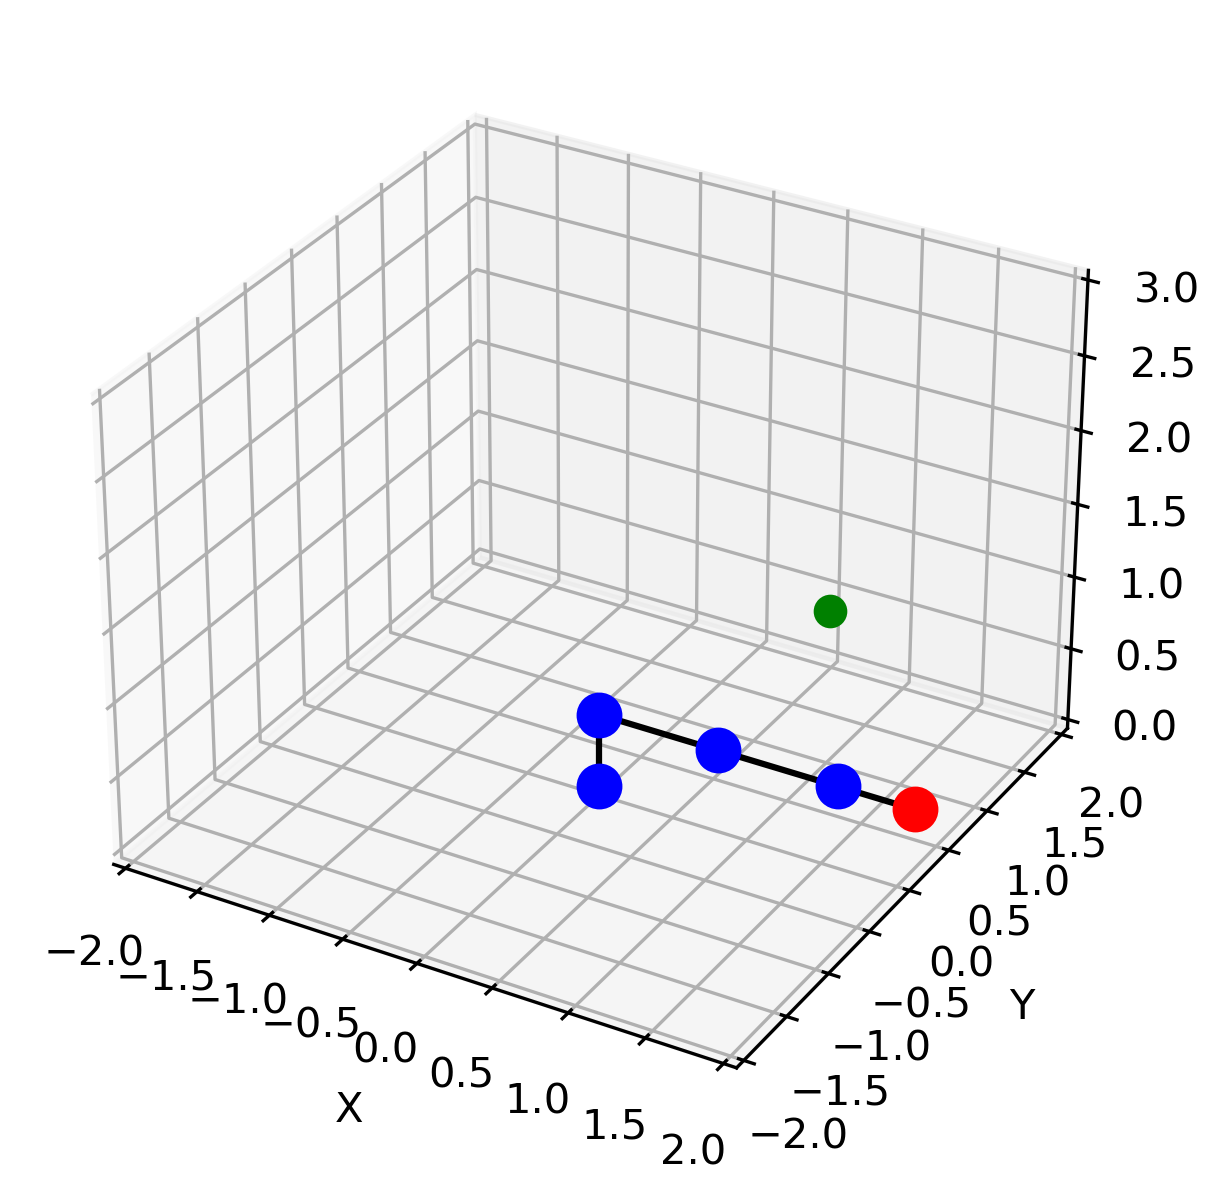
\includegraphics[width=0.5\linewidth]{../robot.png}}
		\caption{ساختار ربات و محیط}
		\label{fig:robot}
	\end{figure}
	برای تعریف این ربات به محیط، از جایی که تنها تغییر زاویه و رسیدن به هدف اهمیت دارد، نوشتن سینماتیک مستقیم ربات کافی است. بنابراین سینماتیک مستقیم این ربات برای هر یک از مفصل‌ها تا انتهای ربات به صورت زیر قابل تعریف می‌باشد.
\begin{equation}
	\begin{aligned}
		x &= \cos(\theta_0) \left( L_1 \cos(\theta_1) + L_2 \cos(\theta_1 + \theta_2) + L_3 \cos(\theta_1 + \theta_2 + \theta_3) \right) \\
		y &= \sin(\theta_0) \left( L_1 \cos(\theta_1) + L_2 \cos(\theta_1 + \theta_2) + L_3 \cos(\theta_1 + \theta_2 + \theta_3) \right) \\
		z &= L_0 + L_1 \sin(\theta_1) + L_2 \sin(\theta_1 + \theta_2) + L_3 \sin(\theta_1 + \theta_2 + \theta_3)
	\end{aligned}
\end{equation}\\
ساختار پاداش‌دهی نیز در 
\autoref{tab:rewarding}
آمده است.
	\begin{table}[h!]
	\caption{نحوه پاداش‌دهی به عامل}
	\begin{latin}
		\centering
		\begin{tabular}{|l|c|}
			\hline
			\textbf{Action result} &  \textbf{Reward} \\ \hline
			Distance to target decreases &  +1  \\  \hline
			Getting close to obstacle &  -1000  \\  \hline
			Reaching target &  +10000 \\ \hline
			Each step &  -1 \\ \hline
		\end{tabular}
	\end{latin}
	\label{tab:rewarding} 
\end{table}\\

\section{یادگیری Q}
حال با سیاست 
\lr{Epsilon-Greedy}
و با
 $\epsilon = 0.3$
 عامل را تربیت می‌کنیم. تربیت برا ۱۰۰۰ اپیزود انجام می‌شود و در نهایت ۳۸ درصد ایپزود‌ها موفق بوده و نمودار پاداش‌های دریافتی در اپیزود‌های موفق در 
 \autoref{fig:Q_rewards}
 آمده است.
 	\begin{figure}[!h]
 	\centerline{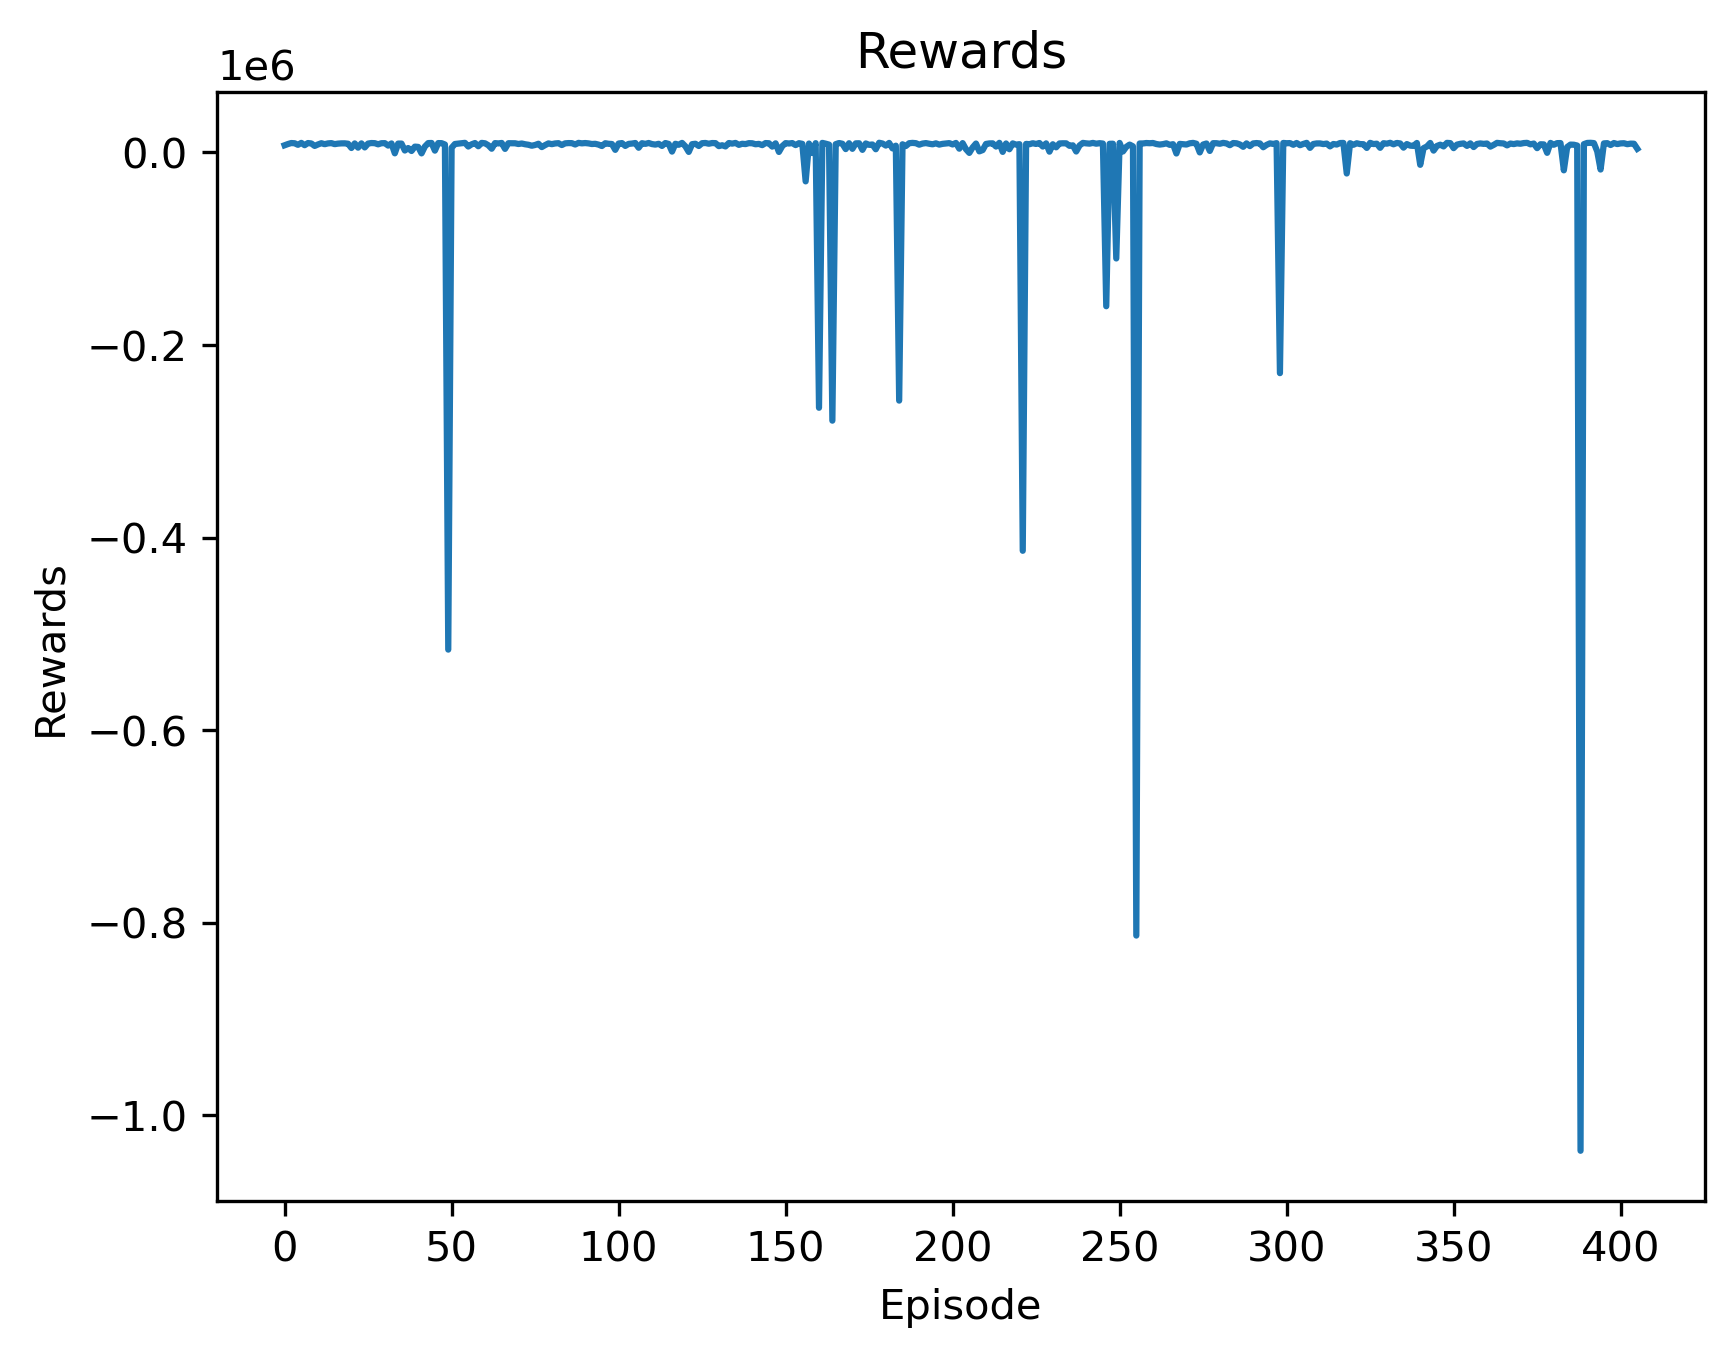
\includegraphics[width=0.5\linewidth]{../Qrewards.png}}
 	\caption{مجموع پاداش‌های اپیزود‌های موفق}
 	\label{fig:Q_rewards}
 \end{figure}
 	\begin{figure}[!h]
 	\centerline{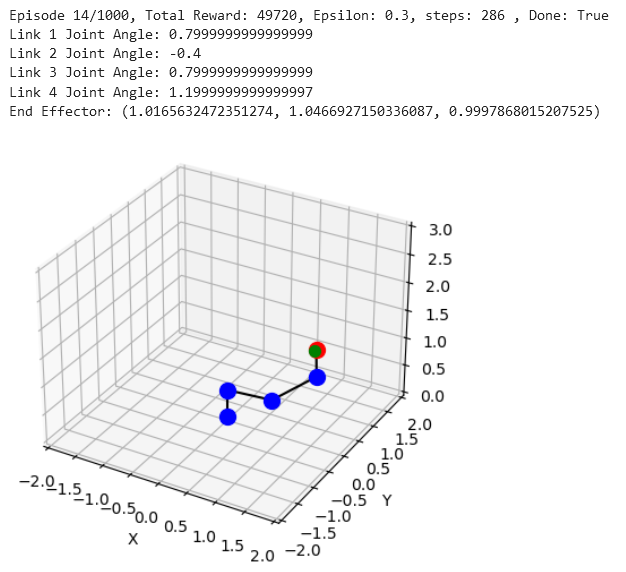
\includegraphics[width=0.5\linewidth]{../success.png}}
 	\caption{یک نمونه از اپیزود‌های موفق}
 	\label{fig:success}
 \end{figure}
\end{document} 